
\documentclass{beamer}
\usepackage[latin1]{inputenc}
%\usetheme{Montpellier}
%\usetheme{Boadilla}
%\usecolortheme[RGB={204,51,255}]{structure}
%\usecolortheme[named=purple]{structure}
\usecolortheme[RGB={62,128,62}]{structure}
%\definecolor{dark}{rgb}{0.3,0.15,0.3}
%\definecolor{light}{rgb}{0.8,0.6,0.8}
%\definecolor{reddish}{rgb}{.5,0.15,0.15}
\definecolor{dark}{rgb}{0.5,0.3,0.4}
%\definecolor{light}{rgb}{0.8,0.6,0.8}
\definecolor{reddish}{rgb}{.7,0.25,0.25}
\definecolor{greenish}{rgb}{.25,0.7,0.25}
\definecolor{blueish}{rgb}{.25,0.25,0.7}
\definecolor{purple}{rgb}{.5,0.0,0.5}
\usepackage{graphicx}
\usepackage{pstricks}

\setbeamertemplate{navigation symbols}{}

\newcommand{\crish}{\color{reddish}}
\newcommand{\cbla}{\color{black}}
\newcommand{\cred}{\color{red}}
\newcommand{\cblu}{\color{blue}}

\usepackage{tikz}
\usetikzlibrary{arrows,decorations.markings,positioning}
\usepackage{epstopdf}




\tikzset{
    state/.style={
           rectangle,
           rounded corners,
           draw=black, very thick,
           inner sep=2pt,
           text centered,
           },
}
\tikzset{
    on/.style={
           circle,
           draw=red, very thick,
           inner sep=2pt,
           fill=red!25,
           },
}


\tikzset{
    off/.style={
           circle,
           draw=blue, very thick,
           inner sep=2pt,
           text centered,
           },
}


\title[Computational Neuroscience 2]{Computational Neuroscience 2}
\author{PHPH20007}
\institute{\texttt{github.com/conorhoughton/PHPH20007}}
\date{April 2020}

\begin{document}

\maketitle

\begin{frame}{Modelling}
This is an example of a model that explains what might be happening without giving a detailed simulation of the individual components involved.
  \end{frame}

\begin{frame}{Modelling}
  Here we look at the hippocampus and introduce a more top down style
  of modelling.
\end{frame}
  
\begin{frame}{The hippocampus}
  \begin{center}
    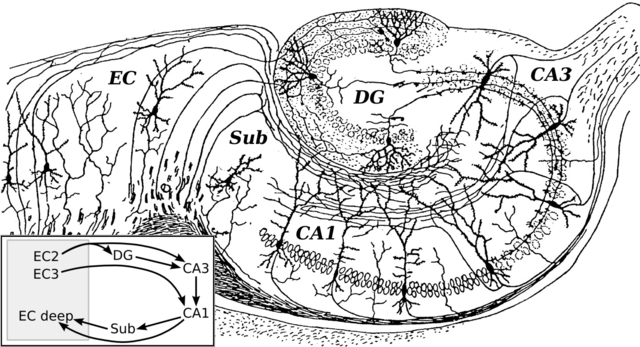
\includegraphics[height=6cm]{hippocampus.png}
  \end{center}
      \vfill
  \flushright{\tiny{image from wikipedia, originally due to Cajal}}
\end{frame}

\begin{frame}{The role of the hippocampus}
  \begin{center}
    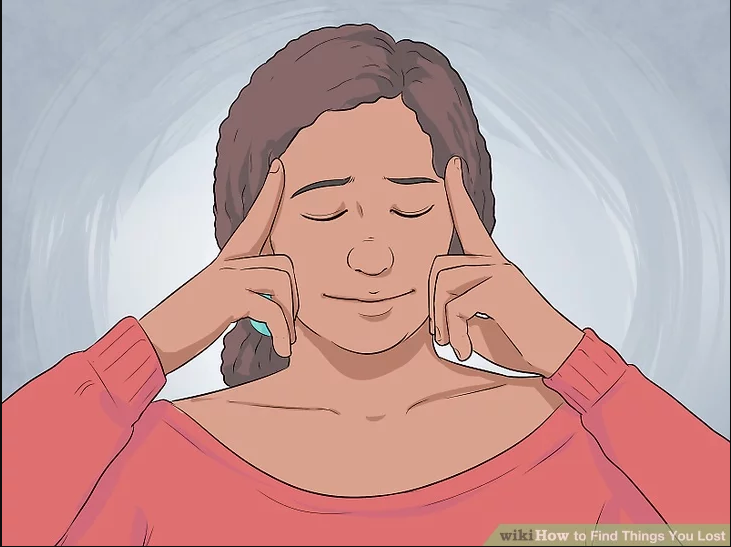
\includegraphics[height=6cm]{finding_lost_items.png}
  \end{center}
      \vfill
  \flushright{\tiny{www.wikihow.life/Find-Things-You-Lost}}
\end{frame}


\begin{frame}{The role of the hippocampus}
  \begin{center}
    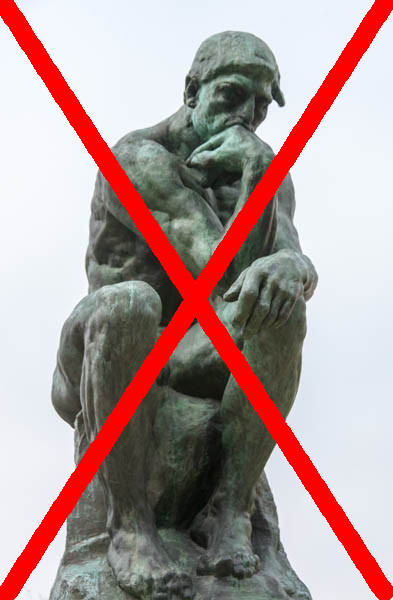
\includegraphics[height=6cm]{the_thinker_cancelled.jpg}
  \end{center}
      \vfill
  \flushright{\tiny{image of Rodin's \textsl{The Thinker} from wikipedia}}
\end{frame}

  
\begin{frame}{The hippocampus}
  \begin{center}
    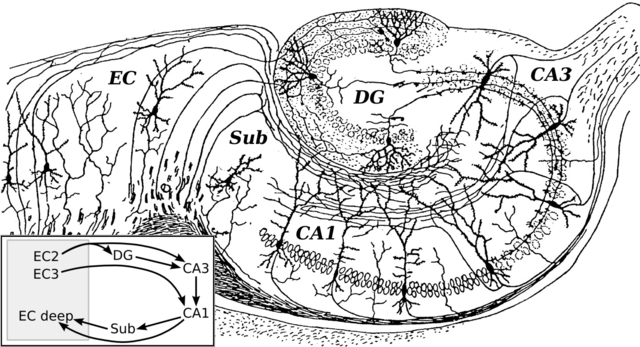
\includegraphics[height=6cm]{hippocampus.png}
  \end{center}
      \vfill
  \flushright{\tiny{image from wikipedia, originally due to Cajal}}
\end{frame}



\begin{frame}{The hippocampus}
\color{red}\textbf{Cornu Ammonis (CA)} - meaning the \textsl{horn of Ammon}. The CA is usually divided
  into four regions, labelled CA1 through to CA4.\color{black}
  \begin{center}
    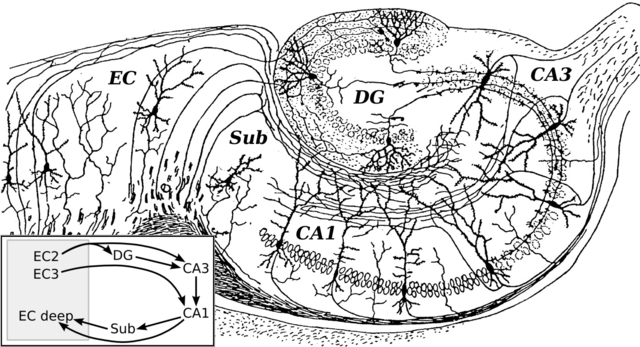
\includegraphics[height=6cm]{hippocampus.png}
  \end{center}
      \vfill
  \flushright{\tiny{image from wikipedia, originally due to Cajal}}
\end{frame}


\begin{frame}{The hippocampus}
\color{red}\textbf{Cornu Ammonis (CA)} - meaning the \textsl{horn of Ammon}. The CA is usually divided
  into four regions, labelled CA1 through to CA4 - sort of.\color{black}
  \begin{center}
    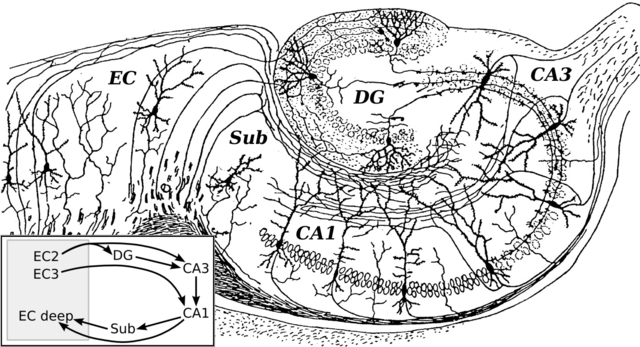
\includegraphics[height=6cm]{hippocampus.png}
  \end{center}
      \vfill
  \flushright{\tiny{image from wikipedia, originally due to Cajal}}
\end{frame}


\begin{frame}{The hippocampus}
\color{red}\textbf{Dentate Gyrus (DG)}- gyrus is the name given to the ridges in the
  cortex, dentate means \textsl{with teeth}.\color{black}
  \begin{center}
    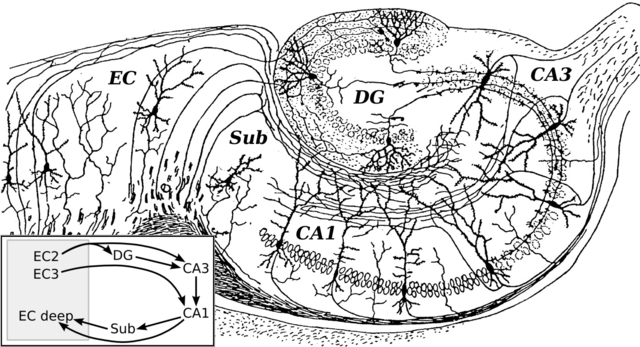
\includegraphics[height=6cm]{hippocampus.png}
  \end{center}
      \vfill
  \flushright{\tiny{image from wikipedia, originally due to Cajal}}
\end{frame}


\begin{frame}{The hippocampus}
\color{red}\textbf{Entorhinal Cortex (EC)} - entorhinal means \textsl{near the smell processing area} - an honorary part of the hippocampus.\color{black}
  \begin{center}
    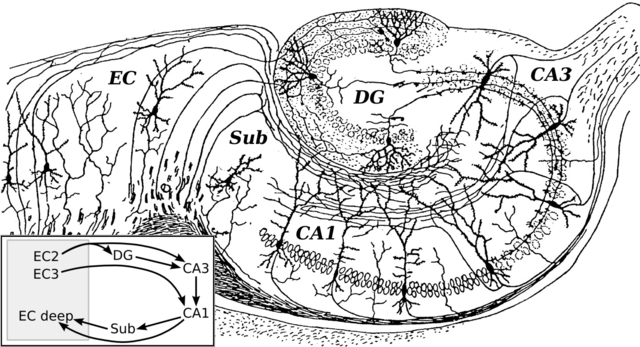
\includegraphics[height=6cm]{hippocampus.png}
  \end{center}
      \vfill
  \flushright{\tiny{image from wikipedia, originally due to Cajal}}
\end{frame}

\begin{frame}{How the hippocampus is connected}
  \begin{center}
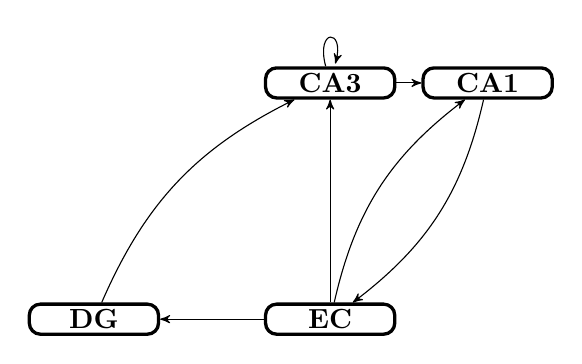
\begin{tikzpicture}[->,>=stealth']

 \node[state,text width=1.5cm](DG) 
 {\textbf{DG}
  };
  
 \node[state, 
 node distance=3cm,
 text width=1.5cm,  
 right of=DG,     
 yshift=+3cm](CA3)
 {\textbf{CA3}
 };
 
 \node[state,
  below of=CA3,
  yshift=-2cm,
  anchor=center,
  text width=1.5cm] (EC) 
 {\textbf{EC}
 };

 \node[state,
  right of=CA3,
  node distance=2cm,
  anchor=center,
text width=1.5cm] (CA1) 
 {\textbf{CA1}
 };

 \path (DG) 	edge[bend left=20]  (CA3)
       (EC)  edge (DG)
 (EC)  edge (CA3)
 (EC)  edge[bend left=20] (CA1)
 (CA1)  edge[bend left=20] (EC)
 (CA3)  edge (CA1)
 (CA3)  	edge[loop above]   (CA3)
;
\end{tikzpicture}
\end{center}
\end{frame}

\begin{frame}{Cells}
  The dentate gyrus is composed of granule cells, CA3 of pyramidal cells. DG is thought of a \textsl{feed-forward} whereas CA3 is highly \textsl{recurrent}.
  \begin{center}
    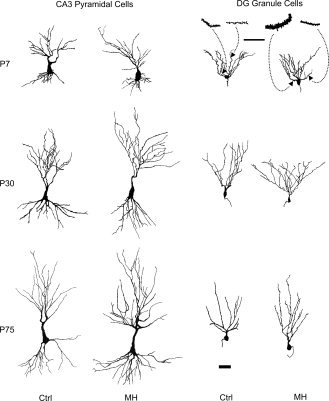
\includegraphics[height=6cm]{cells.jpg}
  \end{center}
      \vfill
  \flushright{\tiny{from 10.1002/jnr.21580}}
\end{frame}

\begin{frame}{Auto-associative memory}

A memory is a pattern of active neurons!
  \begin{center}

\begin{tikzpicture}
\filldraw[color=red!60, fill=red!25, very thick](0,0) circle (.25);
\filldraw[color=blue!60, fill=red!0, very thick](1,0) circle (.25);
\filldraw[color=red!60, fill=red!25, very thick](2,0) circle (.25);
\filldraw[color=blue!60, fill=red!0, very thick](3,0) circle (.25);
\filldraw[color=blue!60, fill=red!0, very thick](4,0) circle (.25);
\filldraw[color=red!60, fill=red!25, very thick](5,0) circle (.25);
\filldraw[color=blue!60, fill=red!0, very thick](6,0) circle (.25);
\filldraw[color=blue!60, fill=red!0, very thick](7,0) circle (.25);
\filldraw[color=blue!60, fill=red!0, very thick](8,0) circle (.25);
\end{tikzpicture}
\end{center}
 \end{frame}


\begin{frame}{Auto-associative memory}

The dynamics of the network complete partial patterns.

\begin{center}
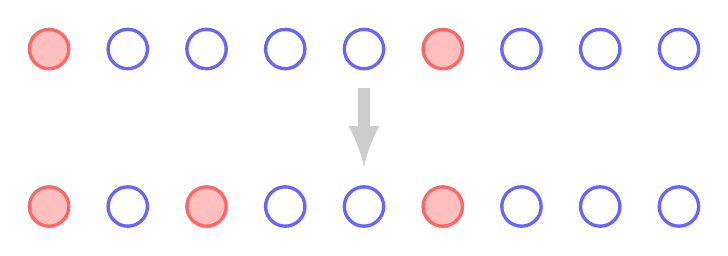
\begin{tikzpicture}
\filldraw[color=red!60, fill=red!25, very thick](0,2) circle (.25);
\filldraw[color=blue!60, fill=red!0, very thick](1,2) circle (.25);
\filldraw[color=blue!60, fill=red!0, very thick](2,2) circle (.25);
\filldraw[color=blue!60, fill=red!0, very thick](3,2) circle (.25);
\filldraw[color=blue!60, fill=red!0, very thick](4,2) circle (.25);
\filldraw[color=red!60, fill=red!25, very thick](5,2) circle (.25);
\filldraw[color=blue!60, fill=red!0, very thick](6,2) circle (.25);
\filldraw[color=blue!60, fill=red!0, very thick](7,2) circle (.25);
\filldraw[color=blue!60, fill=red!0, very thick](8,2) circle (.25);
\coordinate (a) at (4,1.5);
\coordinate (b) at (4,0.5);
\draw[->, >=latex, black!20!white, line width=4pt]   (a) to (b) ;
\filldraw[color=red!60, fill=red!25, very thick](0,0) circle (.25);
\filldraw[color=blue!60, fill=red!0, very thick](1,0) circle (.25);
\filldraw[color=red!60, fill=red!25, very thick](2,0) circle (.25);
\filldraw[color=blue!60, fill=red!0, very thick](3,0) circle (.25);
\filldraw[color=blue!60, fill=red!0, very thick](4,0) circle (.25);
\filldraw[color=red!60, fill=red!25, very thick](5,0) circle (.25);
\filldraw[color=blue!60, fill=red!0, very thick](6,0) circle (.25);
\filldraw[color=blue!60, fill=red!0, very thick](7,0) circle (.25);
\filldraw[color=blue!60, fill=red!0, very thick](8,0) circle (.25);
\end{tikzpicture}
\end{center}

\end{frame}

\begin{frame}{McCulloch-Pitts neurons}
ON!
\begin{center}

\begin{tikzpicture}
\filldraw[color=red!60, fill=red!25, very thick](0,2) circle (.25);
\end{tikzpicture}
\end{center}
\end{frame}

\begin{frame}{McCulloch-Pitts neurons}
OFF!
\begin{center}

\begin{tikzpicture}
\filldraw[color=red!60, fill=red!0, very thick](0,2) circle (.25);
\end{tikzpicture}
\end{center}
\end{frame}

\begin{frame}{All-to-all network}
\begin{center}
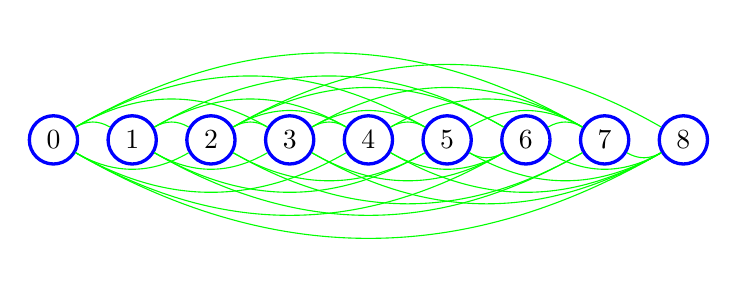
\begin{tikzpicture}
\node[off,text width=0.35cm](0){0};
\node[off,text width=0.35cm,right of = 0](1){1};
\node[off,text width=0.35cm,right of = 1](2){2};
\node[off,text width=0.35cm,right of = 2](3){3};
\node[off,text width=0.35cm,right of = 3](4){4};
\node[off,text width=0.35cm,right of = 4](5){5};
\node[off,text width=0.35cm,right of = 5](6){6};
\node[off,text width=0.35cm,right of = 6](7){7};
\node[off,text width=0.35cm,right of = 7](8){8};
\path (0) edge[bend left,color=green] (1);
\path (0) edge[bend right,color=green] (2);
\path (0) edge[bend left,color=green] (3);
\path (0) edge[bend right,color=green] (4);
\path (0) edge[bend left,color=green] (5);
\path (0) edge[bend right,color=green] (6);
\path (0) edge[bend left,color=green]  (7);
\path (0) edge[bend right,color=green] (8);
\path (1) edge[bend left,color=green] (2);
\path (1) edge[bend right,color=green] (3);
\path (1) edge[bend left,color=green] (4);
\path (1) edge[bend right,color=green] (5);
\path (1) edge[bend left,color=green] (6);
\path (1) edge[bend right,color=green] (7);
\path (2) edge[bend left,color=green] (3);
\path (2) edge[bend left,color=green] (4);
\path (2) edge[bend right,color=green] (5);
\path (2) edge[bend left,color=green] (6);
\path (2) edge[bend right,color=green] (7);
\path (2) edge[bend left,color=green] (8);
\path (3) edge[bend left,color=green] (4);
\path (3) edge[bend left,color=green] (5);
\path (3) edge[bend right,color=green] (6);
\path (3) edge[bend left,color=green] (7);
\path (3) edge[bend right,color=green] (8);
\path (4) edge[bend left,color=green] (5);
\path (4) edge[bend right,color=green] (6);
\path (4) edge[bend left,color=green] (7);
\path (4) edge[bend right,color=green] (8);
\path (5) edge[bend right,color=green] (6);
\path (5) edge[bend left,color=green] (7);
\path (5) edge[bend right,color=green] (8);
\path (6) edge[bend left,color=green] (7);
\path (6) edge[bend right,color=green] (8);
\path (7) edge[bend right,color=green] (8);
\end{tikzpicture}
\end{center}
\end{frame}


\begin{frame}{All-to-all network}
\begin{center}
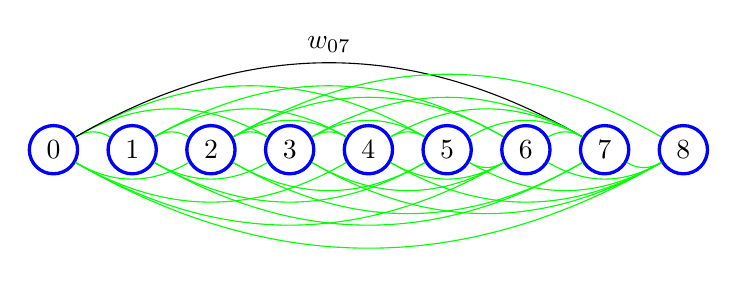
\begin{tikzpicture}
\node[off,text width=0.35cm](0){0};
\node[off,text width=0.35cm,right of = 0](1){1};
\node[off,text width=0.35cm,right of = 1](2){2};
\node[off,text width=0.35cm,right of = 2](3){3};
\node[off,text width=0.35cm,right of = 3](4){4};
\node[off,text width=0.35cm,right of = 4](5){5};
\node[off,text width=0.35cm,right of = 5](6){6};
\node[off,text width=0.35cm,right of = 6](7){7};
\node[off,text width=0.35cm,right of = 7](8){8};
\path (0) edge[bend left,color=green] (1);
\path (0) edge[bend right,color=green] (2);
\path (0) edge[bend left,color=green] (3);
\path (0) edge[bend right,color=green] (4);
\path (0) edge[bend left,color=green] (5);
\path (0) edge[bend right,color=green] (6);
\path (0) edge[bend left,color=black] node[above]{$w_{07}$} (7);
\path (0) edge[bend right,color=green] (8);
\path (1) edge[bend left,color=green] (2);
\path (1) edge[bend right,color=green] (3);
\path (1) edge[bend left,color=green] (4);
\path (1) edge[bend right,color=green] (5);
\path (1) edge[bend left,color=green] (6);
\path (1) edge[bend right,color=green] (7);
\path (2) edge[bend left,color=green] (3);
\path (2) edge[bend left,color=green] (4);
\path (2) edge[bend right,color=green] (5);
\path (2) edge[bend left,color=green] (6);
\path (2) edge[bend right,color=green] (7);
\path (2) edge[bend left,color=green] (8);
\path (3) edge[bend left,color=green] (4);
\path (3) edge[bend left,color=green] (5);
\path (3) edge[bend right,color=green] (6);
\path (3) edge[bend left,color=green] (7);
\path (3) edge[bend right,color=green] (8);
\path (4) edge[bend left,color=green] (5);
\path (4) edge[bend right,color=green] (6);
\path (4) edge[bend left,color=green] (7);
\path (4) edge[bend right,color=green] (8);
\path (5) edge[bend right,color=green] (6);
\path (5) edge[bend left,color=green] (7);
\path (5) edge[bend right,color=green] (8);
\path (6) edge[bend left,color=green] (7);
\path (6) edge[bend right,color=green] (8);
\path (7) edge[bend right,color=green] (8);
\end{tikzpicture}
\end{center}
\end{frame}



\begin{frame}{All-to-all network}
\begin{center}
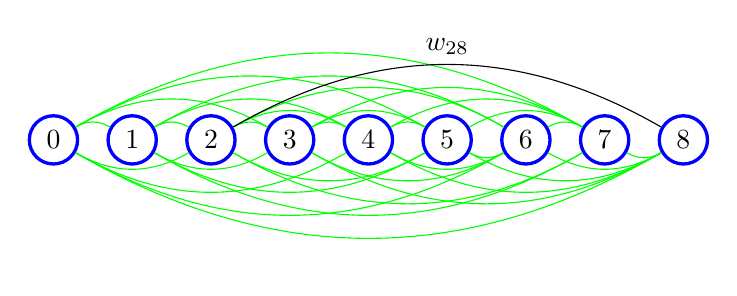
\begin{tikzpicture}
\node[off,text width=0.35cm](0){0};
\node[off,text width=0.35cm,right of = 0](1){1};
\node[off,text width=0.35cm,right of = 1](2){2};
\node[off,text width=0.35cm,right of = 2](3){3};
\node[off,text width=0.35cm,right of = 3](4){4};
\node[off,text width=0.35cm,right of = 4](5){5};
\node[off,text width=0.35cm,right of = 5](6){6};
\node[off,text width=0.35cm,right of = 6](7){7};
\node[off,text width=0.35cm,right of = 7](8){8};
\path (0) edge[bend left,color=green] (1);
\path (0) edge[bend right,color=green] (2);
\path (0) edge[bend left,color=green] (3);
\path (0) edge[bend right,color=green] (4);
\path (0) edge[bend left,color=green] (5);
\path (0) edge[bend right,color=green] (6);
\path (0) edge[bend left,color=green] (7);
\path (0) edge[bend right,color=green] (8);
\path (1) edge[bend left,color=green] (2);
\path (1) edge[bend right,color=green] (3);
\path (1) edge[bend left,color=green] (4);
\path (1) edge[bend right,color=green] (5);
\path (1) edge[bend left,color=green] (6);
\path (1) edge[bend right,color=green] (7);
\path (2) edge[bend left,color=green] (3);
\path (2) edge[bend left,color=green] (4);
\path (2) edge[bend right,color=green] (5);
\path (2) edge[bend left,color=green] (6);
\path (2) edge[bend right,color=green] (7);
\path (2) edge[bend left,color=black]  node[above]{$w_{28}$} (8);
\path (3) edge[bend left,color=green] (4);
\path (3) edge[bend left,color=green] (5);
\path (3) edge[bend right,color=green] (6);
\path (3) edge[bend left,color=green] (7);
\path (3) edge[bend right,color=green] (8);
\path (4) edge[bend left,color=green] (5);
\path (4) edge[bend right,color=green] (6);
\path (4) edge[bend left,color=green] (7);
\path (4) edge[bend right,color=green] (8);
\path (5) edge[bend right,color=green] (6);
\path (5) edge[bend left,color=green] (7);
\path (5) edge[bend right,color=green] (8);
\path (6) edge[bend left,color=green] (7);
\path (6) edge[bend right,color=green] (8);
\path (7) edge[bend right,color=green] (8);
\end{tikzpicture}
\end{center}
\end{frame}

\begin{frame}{Hebbian learning}
  \color{reddish}
  $$
\Delta w_{ij}=\eta (x_i-a)(x_j-a)
$$
\color{black}
where \color{reddish}$a$\color{black} is the average number of ON nodes.
\end{frame}  



\begin{frame}{Hebbian learning}
  \color{reddish}
  $$
\Delta w_{ij}=\eta (x_i-a)(x_j-a)
$$
\color{black}
OFF-OFF causes a small increase
  \color{reddish}
  $$
\Delta w_{01}=\eta a^2
$$
\color{black}
\begin{center}
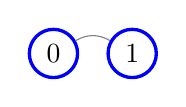
\begin{tikzpicture}
\node[off,text width=0.35cm](0){0};
\node[off,text width=0.35cm,right of = 0](1){1};
\path (0) edge[bend left,color=gray] (1);
\end{tikzpicture}
\end{center}
\end{frame}


\begin{frame}{Hebbian learning}
  \color{reddish}
  $$
\Delta w_{ij}=\eta (x_i-a)(x_j-a)
$$
\color{black}
OFF-ON causes a medium decrease
  \color{reddish}
  $$
\Delta w_{01}=-\eta (1-a)a
$$
\color{black}
\begin{center}
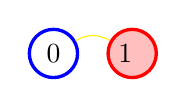
\begin{tikzpicture}
\node[off,text width=0.35cm](0){0};
\node[on,text width=0.35cm,right of = 0](1){1};
\path (0) edge[bend left,color=yellow] (1);
\end{tikzpicture}
\end{center}
\end{frame}


\begin{frame}{Hebbian learning}
  \color{reddish}
  $$
\Delta w_{ij}=\eta (x_i-a)(x_j-a)
$$
\color{black}
ON-ON causes a big increase
  \color{reddish}
  $$
\Delta w_{01}=-\eta (1-a)^2
$$
\color{black}
\begin{center}
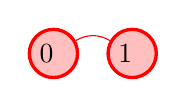
\begin{tikzpicture}
\node[on,text width=0.35cm](0){0};
\node[on,text width=0.35cm,right of = 0](1){1};
\path (0) edge[bend left,color=red] (1);
\end{tikzpicture}
\end{center}
\end{frame}


\begin{frame}{Learning a pattern}
\begin{center}
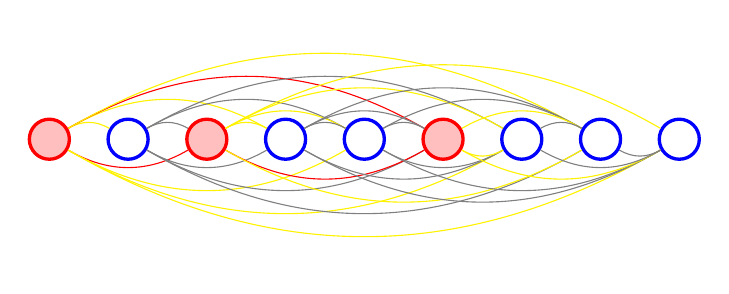
\begin{tikzpicture}
\node[on,text width=0.35cm](0){};
\node[off,text width=0.35cm,right of = 0](1){};
\node[on,text width=0.35cm,right of = 1](2){};
\node[off,text width=0.35cm,right of = 2](3){};
\node[off,text width=0.35cm,right of = 3](4){};
\node[on,text width=0.35cm,right of = 4](5){};
\node[off,text width=0.35cm,right of = 5](6){};
\node[off,text width=0.35cm,right of = 6](7){};
\node[off,text width=0.35cm,right of = 7](8){};
\path (0) edge[bend left,color=yellow] (1);
\path (0) edge[bend right,color=red] (2);
\path (0) edge[bend left,color=yellow] (3);
\path (0) edge[bend right,color=yellow] (4);
\path (0) edge[bend left,color=red] (5);
\path (0) edge[bend right,color=yellow] (6);
\path (0) edge[bend left,color=yellow] (7);
\path (0) edge[bend right,color=yellow] (8);
\path (1) edge[bend left,color=gray] (2);
\path (1) edge[bend right,color=gray] (3);
\path (1) edge[bend left,color=gray] (4);
\path (1) edge[bend right,color=gray] (5);
\path (1) edge[bend left,color=gray] (6);
\path (1) edge[bend right,color=gray] (7);
\path (2) edge[bend left,color=yellow] (3);
\path (2) edge[bend left,color=yellow] (4);
\path (2) edge[bend right,color=red] (5);
\path (2) edge[bend left,color=yellow] (6);
\path (2) edge[bend right,color=yellow] (7);
\path (2) edge[bend left,color=yellow] (8);
\path (3) edge[bend left,color=gray] (4);
\path (3) edge[bend left,color=gray] (5);
\path (3) edge[bend right,color=gray] (6);
\path (3) edge[bend left,color=gray] (7);
\path (3) edge[bend right,color=gray] (8);
\path (4) edge[bend left,color=gray] (5);
\path (4) edge[bend right,color=gray] (6);
\path (4) edge[bend left,color=gray] (7);
\path (4) edge[bend right,color=gray] (8);
\path (5) edge[bend right,color=yellow] (6);
\path (5) edge[bend left,color=yellow] (7);
\path (5) edge[bend right,color=yellow] (8);
\path (6) edge[bend left,color=gray] (7);
\path (6) edge[bend right,color=gray] (8);
\path (7) edge[bend right,color=gray] (8);
\end{tikzpicture}
\end{center}
\end{frame}

\begin{frame}{Activation}
  \color{reddish}
$$
h_i=\sum{w_{ij}x_j} = w_{i0}x_0+w_{i1}x_1+w_{i2}x_2+\ldots
$$
\color{black}{}and if \color{reddish}$h_i>\theta$\color{black}{} set \color{reddish}$x_i$\color{black}{} to one, otherwise set it to zero.
\end{frame}


\begin{frame}{Auto-associative memory}

\begin{center}
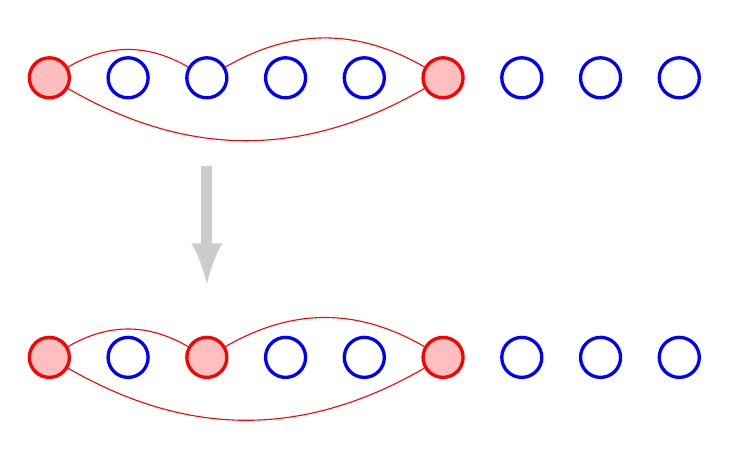
\begin{tikzpicture}
\node[on,text width=0.35cm](0a){};
\node[off,text width=0.35cm,right of = 0a](1a){};
\node[off,text width=0.35cm,right of = 1a](2a){};
\node[off,text width=0.35cm,right of = 2a](3a){};
\node[off,text width=0.35cm,right of = 3a](4a){};
\node[on,text width=0.35cm,right of = 4a](5a){};
\node[off,text width=0.35cm,right of = 5a](6a){};
\node[off,text width=0.35cm,right of = 6a](7a){};
\node[off,text width=0.35cm,right of = 7a](8a){};
\path (0a) edge[bend left,color=red] (2a);
\path (0a) edge[bend right,color=red] (5a);
\path (2a) edge[bend left,color=red] (5a);
\node[below of = 2a](a){};
\node[below = 1.5cm of a](b){};
\draw[->, >=latex, black!20!white, line width=4pt]   (a) to (b) ;
\node[on,text width=0.35cm, below =3cm of 0a](0b){};
\node[off,text width=0.35cm,right of = 0b](1b){};
\node[on,text width=0.35cm,right of = 1b](2b){};
\node[off,text width=0.35cm,right of = 2b](3b){};
\node[off,text width=0.35cm,right of = 3b](4b){};
\node[on,text width=0.35cm,right of = 4b](5b){};
\node[off,text width=0.35cm,right of = 5b](6b){};
\node[off,text width=0.35cm,right of = 6b](7b){};
\node[off,text width=0.35cm,right of = 7b](8b){};
\path (0b) edge[bend left,color=red] (2b);
\path (0b) edge[bend right,color=red] (5b);
\path (2b) edge[bend left,color=red] (5b);

\end{tikzpicture}
\end{center}

\end{frame}

\begin{frame}{Capacity}
  \begin{center}
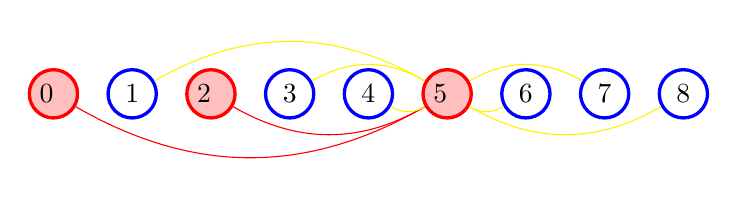
\begin{tikzpicture}
\node[on,text width=0.35cm](0){0};
\node[off,text width=0.35cm,right of = 0](1){1};
\node[on,text width=0.35cm,right of = 1](2){2};
\node[off,text width=0.35cm,right of = 2](3){3};
\node[off,text width=0.35cm,right of = 3](4){4};
\node[on,text width=0.35cm,right of = 4](5){5};
\node[off,text width=0.35cm,right of = 5](6){6};
\node[off,text width=0.35cm,right of = 6](7){7};
\node[off,text width=0.35cm,right of = 7](8){8};
\path (5) edge[bend left,color=red] (0);
\path (5) edge[bend right,color=yellow] (1);
\path (5) edge[bend left,color=red] (2);
\path (5) edge[bend right,color=yellow] (3);
\path (5) edge[bend left,color=yellow] (4);
\path (5) edge[bend right,color=yellow] (6);
\path (5) edge[bend left,color=yellow] (7);
\path (5) edge[bend right,color=yellow] (8);
\end{tikzpicture}
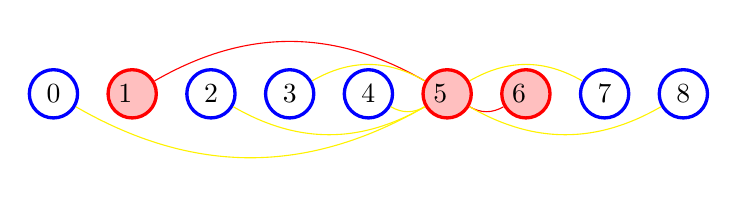
\begin{tikzpicture}
\node[off,text width=0.35cm](0){0};
\node[on,text width=0.35cm,right of = 0](1){1};
\node[off,text width=0.35cm,right of = 1](2){2};
\node[off,text width=0.35cm,right of = 2](3){3};
\node[off,text width=0.35cm,right of = 3](4){4};
\node[on,text width=0.35cm,right of = 4](5){5};
\node[on,text width=0.35cm,right of = 5](6){6};
\node[off,text width=0.35cm,right of = 6](7){7};
\node[off,text width=0.35cm,right of = 7](8){8};
\path (5) edge[bend left,color=yellow] (0);
\path (5) edge[bend right,color=red] (1);
\path (5) edge[bend left,color=yellow] (2);
\path (5) edge[bend right,color=yellow] (3);
\path (5) edge[bend left,color=yellow] (4);
\path (5) edge[bend right,color=red] (6);
\path (5) edge[bend left,color=yellow] (7);
\path (5) edge[bend right,color=yellow] (8);
\end{tikzpicture}
  \end{center}
\end{frame}


\begin{frame}{Capacity}
  \begin{itemize}
  \item \color{reddish}$N^2$\color{black}{} connections.
  \item \color{reddish}$N$\color{black}{} neurons in a pattern.
   \item Can store something proportional to \color{reddish}$N^2/N=N$\color{black}{} patterns.
    \end{itemize}
\end{frame}

\begin{frame}{Correlated patterns}
  \begin{center}
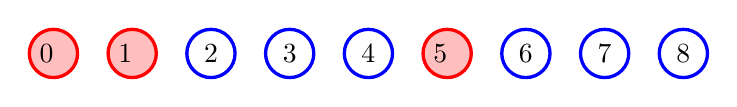
\begin{tikzpicture}
\node[on,text width=0.35cm](0){0};
\node[on,text width=0.35cm,right of = 0](1){1};
\node[off,text width=0.35cm,right of = 1](2){2};
\node[off,text width=0.35cm,right of = 2](3){3};
\node[off,text width=0.35cm,right of = 3](4){4};
\node[on,text width=0.35cm,right of = 4](5){5};
\node[off,text width=0.35cm,right of = 5](6){6};
\node[off,text width=0.35cm,right of = 6](7){7};
\node[off,text width=0.35cm,right of = 7](8){8};
\end{tikzpicture}
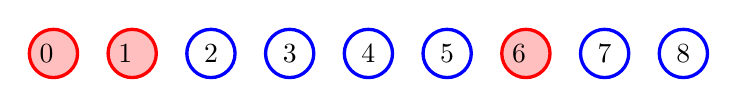
\begin{tikzpicture}
\node[on,text width=0.35cm](0){0};
\node[on,text width=0.35cm,right of = 0](1){1};
\node[off,text width=0.35cm,right of = 1](2){2};
\node[off,text width=0.35cm,right of = 2](3){3};
\node[off,text width=0.35cm,right of = 3](4){4};
\node[off,text width=0.35cm,right of = 4](5){5};
\node[on,text width=0.35cm,right of = 5](6){6};
\node[off,text width=0.35cm,right of = 6](7){7};
\node[off,text width=0.35cm,right of = 7](8){8};
\end{tikzpicture}
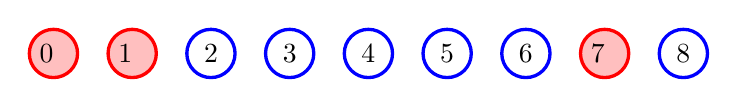
\begin{tikzpicture}
\node[on,text width=0.35cm](0){0};
\node[on,text width=0.35cm,right of = 0](1){1};
\node[off,text width=0.35cm,right of = 1](2){2};
\node[off,text width=0.35cm,right of = 2](3){3};
\node[off,text width=0.35cm,right of = 3](4){4};
\node[off,text width=0.35cm,right of = 4](5){5};
\node[off,text width=0.35cm,right of = 5](6){6};
\node[on,text width=0.35cm,right of = 6](7){7};
\node[off,text width=0.35cm,right of = 7](8){8};
\end{tikzpicture}
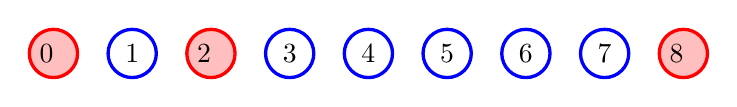
\begin{tikzpicture}
\node[on,text width=0.35cm](0){0};
\node[off,text width=0.35cm,right of = 0](1){1};
\node[on,text width=0.35cm,right of = 1](2){2};
\node[off,text width=0.35cm,right of = 2](3){3};
\node[off,text width=0.35cm,right of = 3](4){4};
\node[off,text width=0.35cm,right of = 4](5){5};
\node[off,text width=0.35cm,right of = 5](6){6};
\node[off,text width=0.35cm,right of = 6](7){7};
\node[on,text width=0.35cm,right of = 7](8){8};
\end{tikzpicture}
  \end{center}
\end{frame}

\begin{frame}{Erroneous completion}
\begin{center}
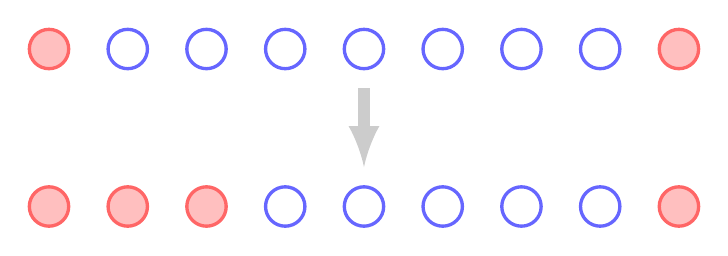
\begin{tikzpicture}
\filldraw[color=red!60, fill=red!25, very thick](0,2) circle (.25);
\filldraw[color=blue!60, fill=red!0, very thick](1,2) circle (.25);
\filldraw[color=blue!60, fill=red!0, very thick](2,2) circle (.25);
\filldraw[color=blue!60, fill=red!0, very thick](3,2) circle (.25);
\filldraw[color=blue!60, fill=red!0, very thick](4,2) circle (.25);
\filldraw[color=blue!60, fill=red!0, very thick](5,2) circle (.25);
\filldraw[color=blue!60, fill=red!0, very thick](6,2) circle (.25);
\filldraw[color=blue!60, fill=red!0, very thick](7,2) circle (.25);
\filldraw[color=red!60, fill=red!25, very thick](8,2) circle (.25);
\coordinate (a) at (4,1.5);
\coordinate (b) at (4,0.5);
\draw[->, >=latex, black!20!white, line width=4pt]   (a) to (b) ;
\filldraw[color=red!60, fill=red!25, very thick](0,0) circle (.25);
\filldraw[color=red!60, fill=red!25, very thick](1,0) circle (.25);
\filldraw[color=red!60, fill=red!25, very thick](2,0) circle (.25);
\filldraw[color=blue!60, fill=red!0, very thick](3,0) circle (.25);
\filldraw[color=blue!60, fill=red!0, very thick](4,0) circle (.25);
\filldraw[color=blue!60, fill=red!0, very thick](5,0) circle (.25);
\filldraw[color=blue!60, fill=red!0, very thick](6,0) circle (.25);
\filldraw[color=blue!60, fill=red!0, very thick](7,0) circle (.25);
\filldraw[color=red!60, fill=red!25, very thick](8,0) circle (.25);
\end{tikzpicture}
\end{center}
or even
\begin{center}
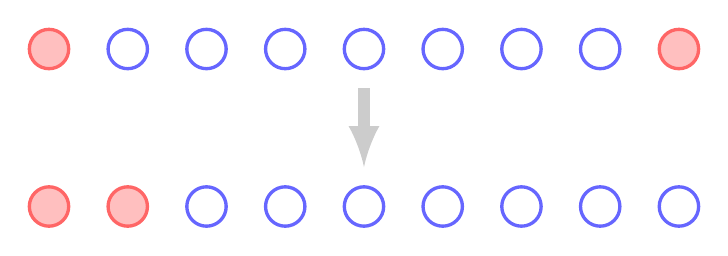
\begin{tikzpicture}
\filldraw[color=red!60, fill=red!25, very thick](0,2) circle (.25);
\filldraw[color=blue!60, fill=red!0, very thick](1,2) circle (.25);
\filldraw[color=blue!60, fill=red!0, very thick](2,2) circle (.25);
\filldraw[color=blue!60, fill=red!0, very thick](3,2) circle (.25);
\filldraw[color=blue!60, fill=red!0, very thick](4,2) circle (.25);
\filldraw[color=blue!60, fill=red!0, very thick](5,2) circle (.25);
\filldraw[color=blue!60, fill=red!0, very thick](6,2) circle (.25);
\filldraw[color=blue!60, fill=red!0, very thick](7,2) circle (.25);
\filldraw[color=red!60, fill=red!25, very thick](8,2) circle (.25);
\coordinate (a) at (4,1.5);
\coordinate (b) at (4,0.5);
\draw[->, >=latex, black!20!white, line width=4pt]   (a) to (b) ;
\filldraw[color=red!60, fill=red!25, very thick](0,0) circle (.25);
\filldraw[color=red!60, fill=red!25, very thick](1,0) circle (.25);
\filldraw[color=blue!60, fill=red!0, very thick](2,0) circle (.25);
\filldraw[color=blue!60, fill=red!0, very thick](3,0) circle (.25);
\filldraw[color=blue!60, fill=red!0, very thick](4,0) circle (.25);
\filldraw[color=blue!60, fill=red!0, very thick](5,0) circle (.25);
\filldraw[color=blue!60, fill=red!0, very thick](6,0) circle (.25);
\filldraw[color=blue!60, fill=red!0, very thick](7,0) circle (.25);
\filldraw[color=blue!60, fill=red!0, very thick](8,0) circle (.25);
\end{tikzpicture}
\end{center}
\end{frame}

\begin{frame}{Patterns seperation}
  Maybe the Dentate Gyrus fixes this problem!
\end{frame}

\begin{frame}{Summary}
\begin{enumerate}
\item CA3 - many recurrent connections, that is excitatory neurons connected to each other.
\item CA3 - an auto-associative memory store - patterns are completed.
\item CA3 - capacity proportional to \color{reddish}$N$\color{black}.
\item DG - feedforward, that is few, or even no, lateral connections between the excitatory neurons.
\item DG - seperates patterns ready for EC to store them by randomizing them.
\end{enumerate}
\end{frame}

\end{document}

